\documentclass[a0paper,portrait]{baposter}

\usepackage{subfigure} 
\usepackage{fontspec} %加這個就可以設定字體
\usepackage{xeCJK} %讓中英文字體分開設置
\setCJKmainfont{標楷體} %設定中文為系統上的字型,而英文不去更動,使用原TeX字型
\XeTeXlinebreaklocale "zh" %這兩行一定要加,中文才能自動換行
\XeTeXlinebreakskip = 0pt plus 1pt %這兩行一定要加,中文才能自動換行

\usepackage[font=small,labelfont=bf]{caption} % Required for specifying captions to tables and figures
\usepackage{booktabs} % Horizontal rules in tables
\usepackage{relsize} % Used for making text smaller in some places
\usepackage{tikz}

\graphicspath{{figures/}} % Directory in which figures are stored

\definecolor{bordercol}{RGB}{40,40,40} % Border color of content boxes
\definecolor{headercol1}{RGB}{186,215,230} % Background color for the header in the content boxes (left side)
\definecolor{headercol2}{RGB}{80,80,80} % Background color for the header in the content boxes (right side)
\definecolor{headerfontcol}{RGB}{0,0,0} % Text color for the header text in the content boxes
\definecolor{boxcolor}{RGB}{186,215,230} % Background color for the content in the content boxes

\begin{document}

\background{ % Set the background to an image (background.pdf)
\begin{tikzpicture}[remember picture,overlay]
\draw (current page.north west)+(-2em,2em) node[anchor=north west]
{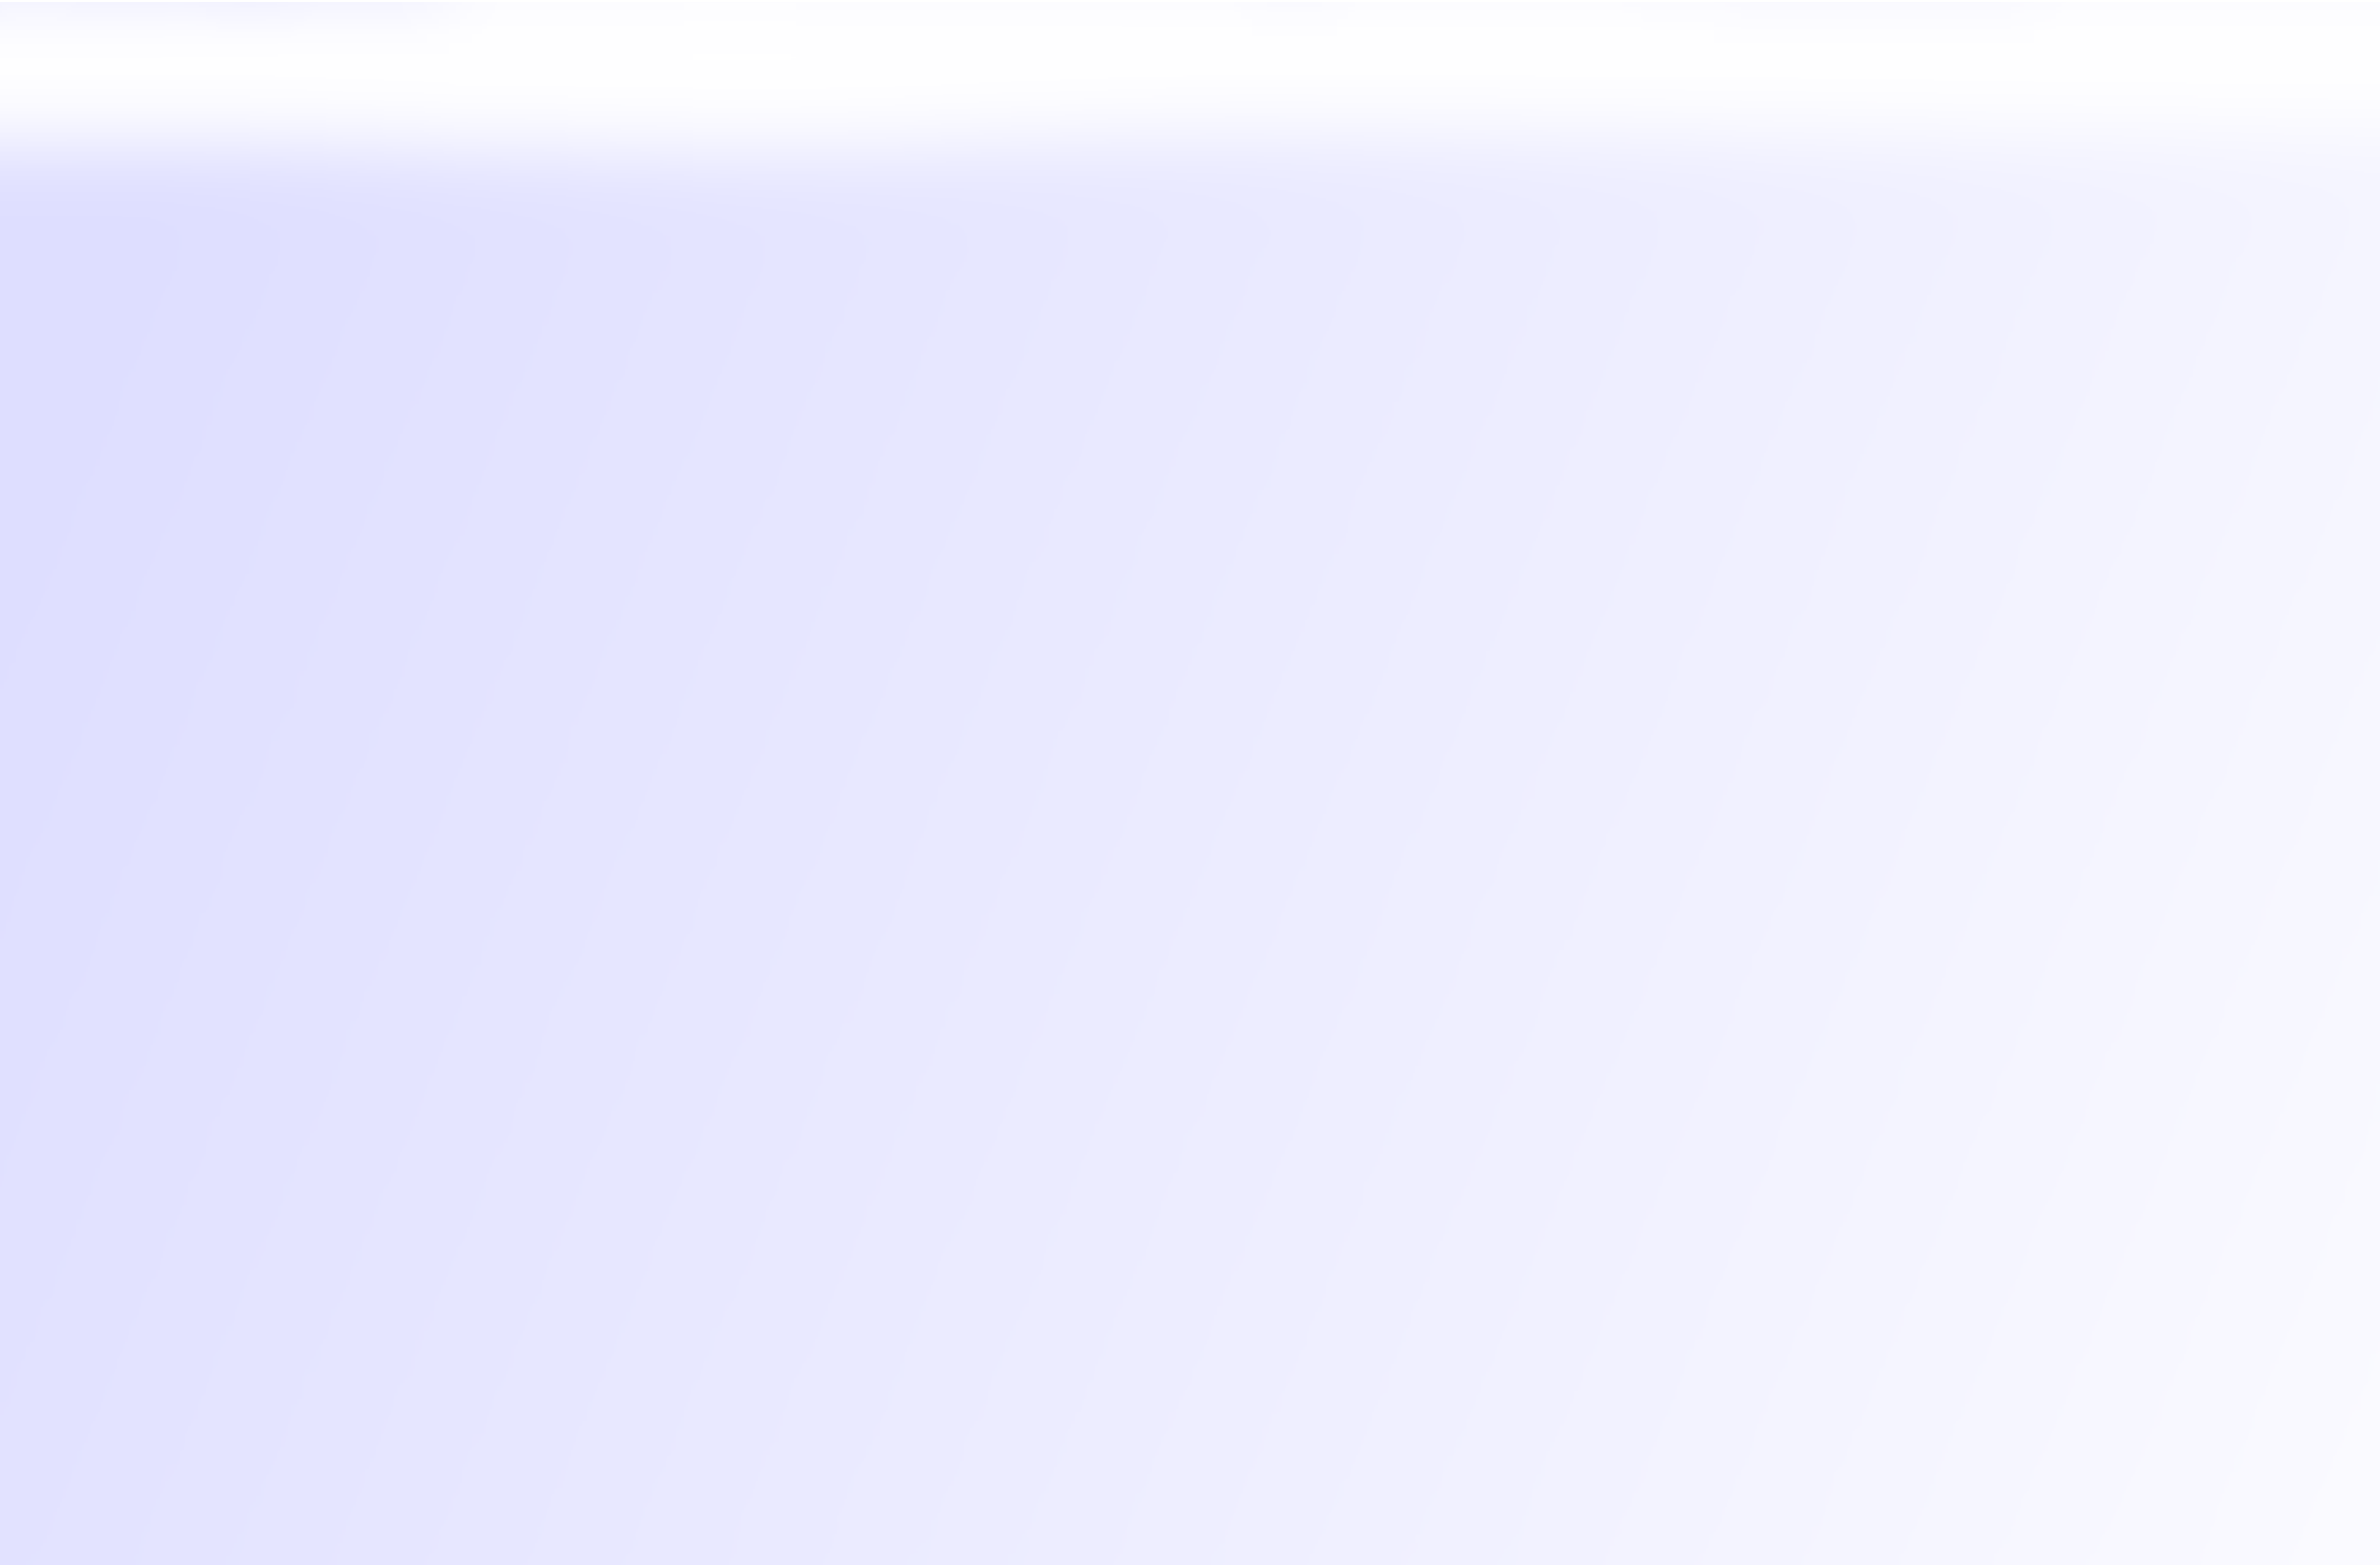
\includegraphics[height=1.1\textheight]{background}};
\end{tikzpicture}
}

\begin{poster}{
columns=2,
grid=false,
borderColor=bordercol, % Border color of content boxes
headerColorOne=headercol1, % Background color for the header in the content boxes (left side)
headerColorTwo=headercol2, % Background color for the header in the content boxes (right side)
headerFontColor=headerfontcol, % Text color for the header text in the content boxes
boxColorOne=boxcolor, % Background color for the content in the content boxes
headershape=roundedright, % Specify the rounded corner in the content box headers
headerfont=\Large\sf\bf, % Font modifiers for the text in the content box headers
textborder=rectangle,
background=user,
headerborder=open, % Change to closed for a line under the content box headers
boxshade=plain
}
{}
%
%----------------------------------------------------------------------------------------
%	TITLE AND AUTHOR NAME
%----------------------------------------------------------------------------------------
%
{\sf\bf AndMuscle \\ \smaller \smaller 基於Android行動裝置與肌肉感測器之 \\ 網路連線即時對戰擴增實境遊戲} % Poster title
%{\sf 基於Android行動裝置與肌肉感測器之網路連線即時對戰擴增實境遊戲}
{\vspace{1em} 指導教授: 張欽圳\space 老師
 \space \space 專題成員: 王佳君 \space 林令婕 % Author names
}
{
\includegraphics[scale=1.0]{ntoulogo}} % University/lab logo

%----------------------------------------------------------------------------------------
%	簡介 INTRODUCTION
%----------------------------------------------------------------------------------------

\headerbox{簡介\space Introduction}
{name=introduction,column=0,row=0}{

本專題設計為一款雙人網路連線即時對戰的擴增實境遊戲,於 Android 行動裝置上開發,結合影像處理及肌肉感測器技術, 以之為主架構來設計。
\\ 在這款遊戲中,利用肌肉感測器測量肌肉活動狀況,及不斷改變肌肉施力大小與頻率,來達成開發者要求。建立網路通道,即時傳輸感測器數據與雙方畫面,以現實中對方遊戲者臉部影像為基礎,改變其皮膚色調,且在指定位置拼貼上逗趣的圖示。
}

%----------------------------------------------------------------------------------------
%	系統架構 System Architecture
%----------------------------------------------------------------------------------------

\headerbox{系統架構\space System Architecture}{name=architecture,column=0,below=introduction}{
遊戲系統分為Android端及肌肉感測器端: Android中主要含網路連線及影像處理兩部分。利用網路連線與伺服器端開啟網路通道,影像處理則透過特徵點的取得在指定的位置上進行圖像修改;肌肉感測器運用Arduino來獲取肌肉數據並以傅立葉轉換分析。Android與肌肉感測器 則是透過藍芽模組串連,完成整個遊戲系統。
\center
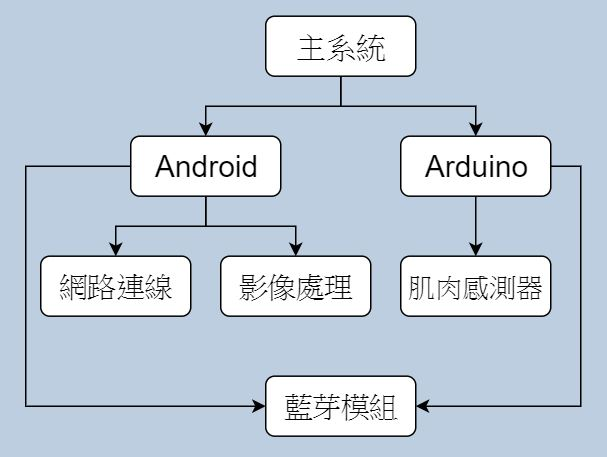
\includegraphics[scale=0.6]{軟硬體架構圖.JPG}

}

%----------------------------------------------------------------------------------------
%	技術說明(一) Technical Description I
%----------------------------------------------------------------------------------------

\headerbox{技術說明\space Technical Description}{name=technical01,column=0,below=architecture}{
\begin{itemize}
\item 網路連線
\begin{description}
\item[1] 基於TCP網路架構,建構出伺服器(Server)端及玩家(Client)端。
\item[2] 透過socket連線後,使用不同Thread分別執行inputstream與outputstream,於網路通道上進行輸入及輸出,且以lock、unlock、await、signal處理同步問題。
\item[3] Client端連線架構圖 \\
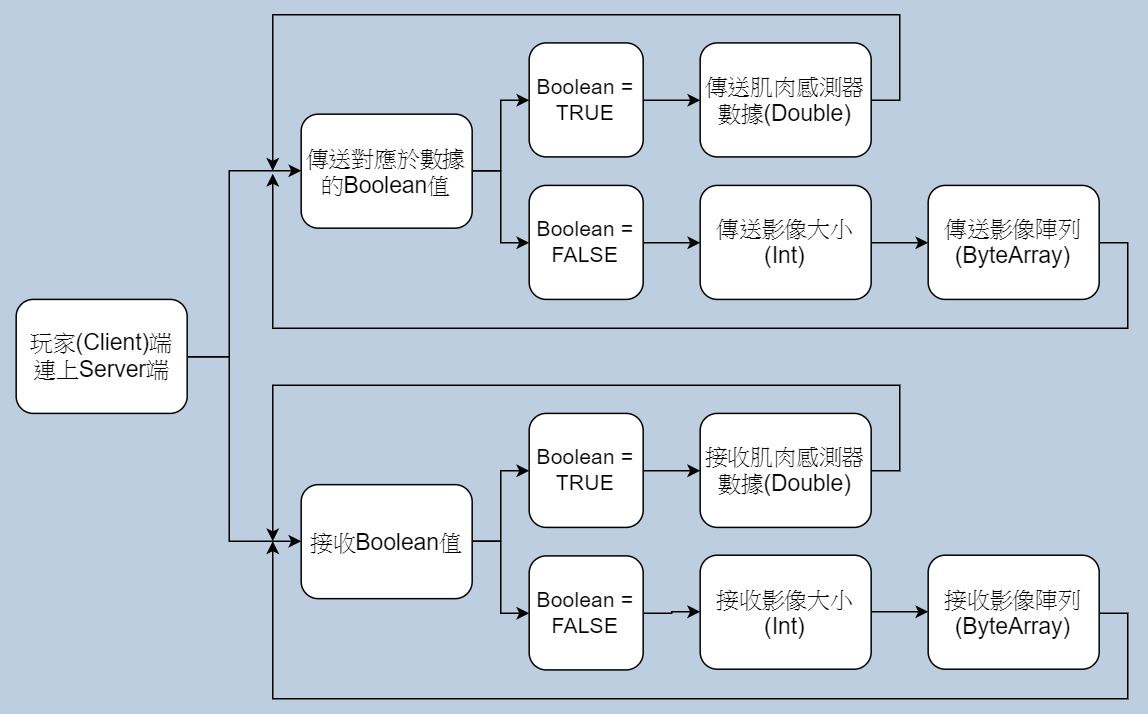
\includegraphics[scale=0.45]{Client.JPG}
\end{description}

\item 臉部偵測
\begin{description}
\item[1] 運用Google Firebase ML Kit 提供之API進行面部特徵點的取得。
\item[2] 在Detector運行前進行Options的設定及欲偵測之檔案型態轉換。
\item[3] 塗鴉後將所塗鴉過之區域進行紀錄,以保存資料。\\
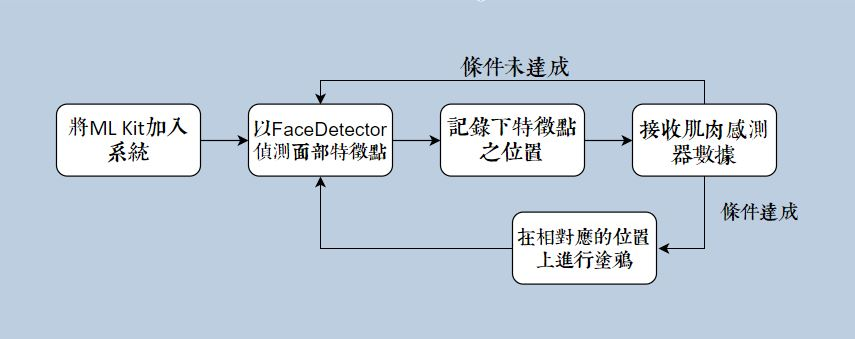
\includegraphics[scale=0.4]{face.JPG}
\end{description}

\end{itemize}
}

%----------------------------------------------------------------------------------------
%	技術說明(二) Technical Description II
%----------------------------------------------------------------------------------------

\headerbox{技術說明\space Technical Description}{name=technical02,column=1,row=0}{
\begin{itemize}
\item 肌肉感測器數據分析
\begin{description}
\item[1] 使用快速傅立葉分析進行數據轉換分析
\item[2] 數據分析架構圖 \\
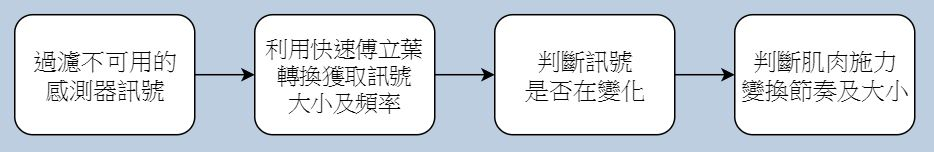
\includegraphics[scale=0.55]{Muscle.JPG}
\end{description}

\end{itemize}
}

%----------------------------------------------------------------------------------------
%	實驗結果 Experiment Result
%----------------------------------------------------------------------------------------

\headerbox{實驗結果\space Experiment Result}{name=experiment,column=1,below=technical02}{

\begin{itemize}
\item 遊戲主頁面及開始畫面(連線上Server) \\ \\
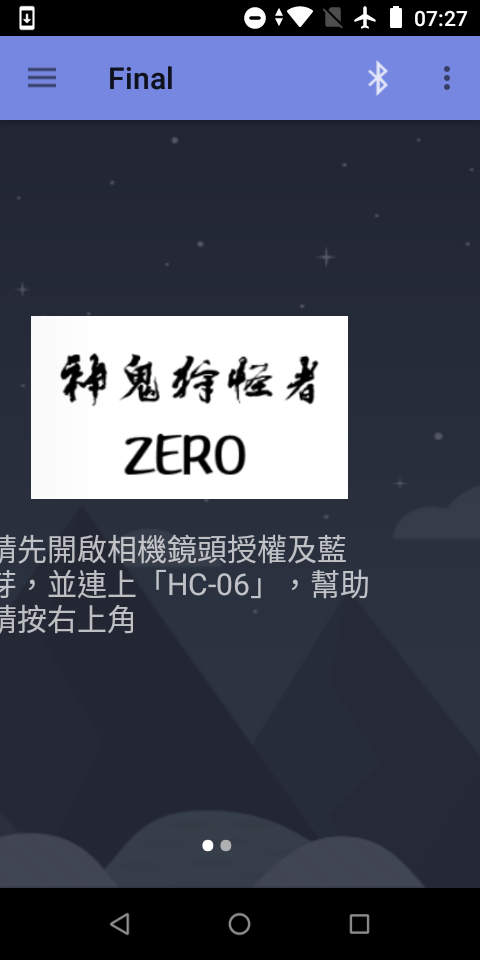
\includegraphics[scale=0.15]{game01.png} 
\space \space
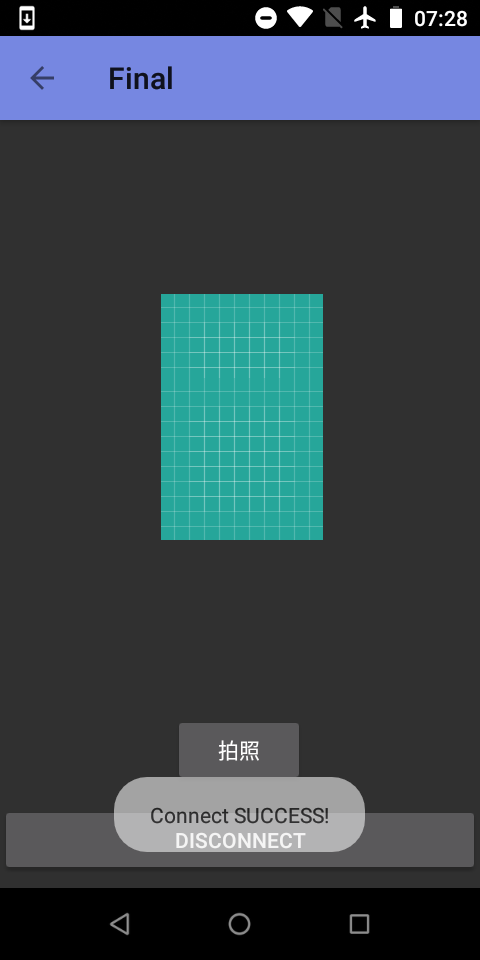
\includegraphics[scale=0.15]{game02.png}
\item 遊戲中畫面 \\ \\
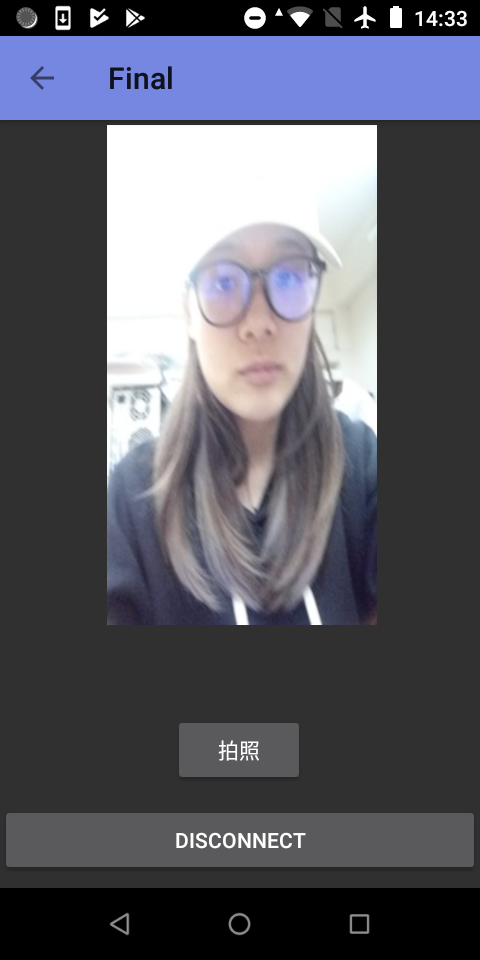
\includegraphics[scale=0.15]{game03.png}
\item 遊戲結束畫面 \\ \\
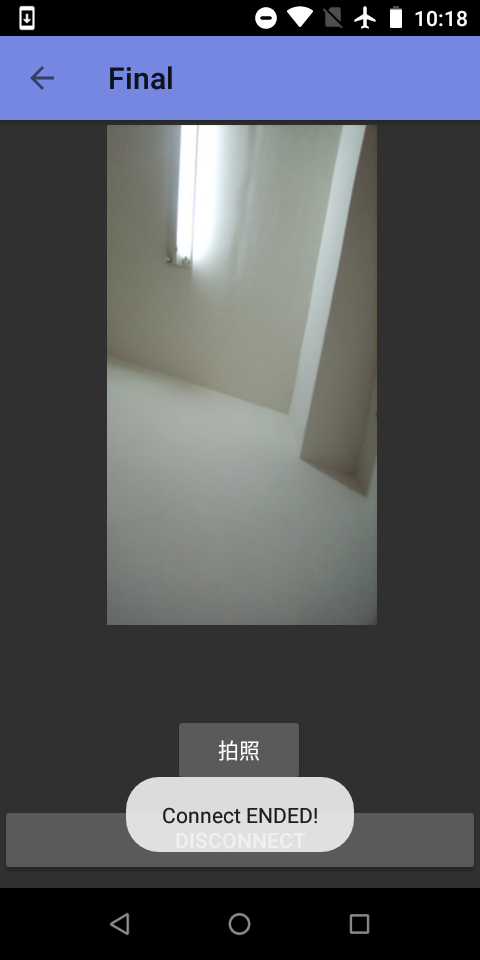
\includegraphics[scale=0.15]{game04.png}
\end{itemize}
}

%----------------------------------------------------------------------------------------
%	結論 Conclusion
%----------------------------------------------------------------------------------------

%\headerbox{結論\space Conclusion}
%{name=conclusion,column=1,below=experiment}{

%結論

%\begin{enumerate}
%\item 第一點
%\item 第二點
%\end{enumerate}
%}

%----------------------------------------------------------------------------------------
%	討論 Discussion
%----------------------------------------------------------------------------------------

\headerbox{討論\space Discussion}{name=discussion,column=1,below=experiment}{

\begin{itemize}
\item 臉部特徵點位置取得上,會因人物的動作而識別出現誤差。
\item 網路傳送影像大小後,為避免此數據與影像數據混淆,會先暫停0.1秒,造成接收效率降低。
\end{itemize}
}

%----------------------------------------------------------------------------------------

\end{poster}

\end{document}